\documentclass{cnbwp}
\usepackage{graphicx}
\usepackage{dcolumn,verbatim}
\usepackage[figuresright]{rotating} % for sideways tables

% End of the preamble

\begin{document}
\title{Sample Template for Writing the Working Papers of the Czech National Bank, a Long Title Is
Used}
\author{Ferdinand Mravenec}{Czech National Bank, Division A, ferda@mravenec.cz}
\author{Brouk Pytl\'ik}{Czech National Bank, Division B, brouk@pytlik.cz}
\author{Beru\v{s}ka Sedmite\v{c}n\'a}{Czech National Bank, Division B, beruska@louka.cz}
\acknowledge{This work was supported by Czech National Bank Research Project No. .\\
The authors would like to thank ...\\
The views expressed in this paper are those of the authors and not necessarily those of the Czech
National Bank.}
\maketitle

\begin{abstract}
This is the template of the Working Papers. This environment should contain the abstract. The JEL
codes and keywords must appear below but after the Czech abstract.
\end{abstract}

\begin{abstrakt}
Toto je \v{c}esk\'y abstrakt k p\v{r}\'ikladu pou\v{z}it\'i \v{s}ablony Working Papers. N\'asleduje po anglick\'em abstraktu,
po n\v{e}m se uvedou k\'ody JEL a kl\'i\v{c}ov\'a slova.
\end{abstrakt}

\JEL{B6, B12, B52, Z80}

\Keywords{Template, working paper, table, figure, references}

\begin{nontechsummary}
This part of the document is devoted to the nontechnical summary.
\end{nontechsummary}

\section{Section}
The document is organized in sections and subsections as shown below.

\subsection{Images}
The images are inserted preferably using the ``graphicx'' package. The caption should be placed
above the picture, see the sample below.

\begin{figure}[hbt]
\caption{Sample of Graphics}
\ifpdf
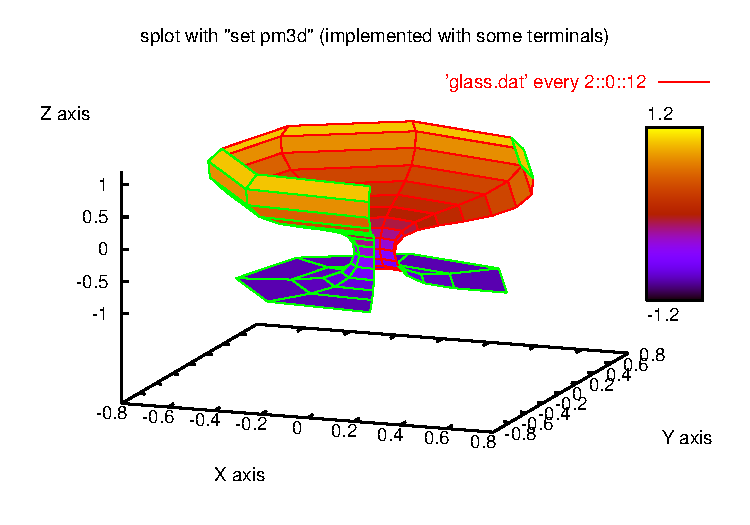
\includegraphics[width=\textwidth]{graph18.pdf}
\else
\includegraphics[width=\textwidth]{graph18.eps}
\fi
\medskip
\Note{This example shows inclusion a vector image.}
\Source{gnuplot}
\end{figure}

\subsection{Numerical Tables}
Numerical tables make use of the ``dcolumn'' package for alignment on the decimal dot. The sample is
given below.

\begin{table}[hbt]
\caption{Numerical table}\medskip
\setlength\extrarowheight{2pt}
\begin{tabular}{|l|D{,}{.}{2}D{,}{.}{1}|}\hline
\bfseries Jm\'eno & \multicolumn{1}{c}{\bfseries V\'y\v{s}ka [m]} &
\multicolumn{1}{c|}{\bfseries V\'aha [kg]}\\\hline
Zlatovl\'aska & 1,68 & 62,3 \\
Dlouh\'y      & 12,6 & 98,1 \\
\v{S}irok\'y  & 1,83 & 386 \\
Bystrozrak\'y & 1,74 & 74,2 \\\hline
\end{tabular}

\end{table}

\subsection{Wide rotated tables}
Wide tables must be rotated. They usually take the whole page.

\begin{sidewaystable}[p]
\setlength{\extrarowheight}{2pt}
\newcommand\mcol[1]{\multicolumn{1}{r}{Col. #1}}
\centeredcaption{\v{S}irok\'a tabulka}\label{widetable}\bigskip\centering
\begin{tabular}{l*{10}{D{.}{.}{3}}}\hline
\bfseries \# &\mcol{1}&\mcol{2}&\mcol{3}&\mcol{4}
&\mcol{5}&\mcol{6}&\mcol{7}&\mcol{8}&\mcol{9}&\mcol{10}\\\hline
Row  1 &  -6.412 &  -2.654 &  -5.300 &   4.358 &  -6.473 &  -4.573 &   2.391 &  -0.497 &  -4.262 &  -0.341\\
Row  2 &   2.799 &  -8.109 &   5.647 &  -0.214 &   4.665 &   2.971 &  13.699 &  -5.059 &  -0.088 &   4.090\\
Row  3 &   8.427 &   5.467 &  -7.061 &  -0.347 &  -6.955 &   6.352 &  -3.955 &   7.768 &  -9.852 &   4.618\\
Row  4 &  -1.978 &  -1.226 &   1.136 &   1.733 &   3.874 &  15.072 &   4.112 &  -1.931 &   4.127 &   1.177\\
Row  5 &  10.896 &   6.859 &  -0.623 &   6.685 &  -6.378 &   2.714 &  -2.670 &   7.862 &  -2.314 &  -4.094\\
Row  6 &  -5.013 &  -2.391 &  -1.763 &  -1.499 &  -4.053 &   2.453 &   1.550 &  -3.939 &   3.366 &  -0.780\\
Row  7 &   8.644 &  -1.787 &  -5.782 &   1.244 &  -0.806 &   3.506 &   1.810 &  -3.908 &  -0.626 &  -1.933\\
Row  8 &  -4.965 &  -2.494 &   1.539 &   6.265 &   0.892 &  -2.730 &   3.311 &  -0.006 &   3.735 &   0.408\\
Row  9 &   1.237 &  -3.029 &  -0.773 &   9.400 &  -6.009 &  -0.487 &   4.281 &   4.520 &  -5.744 &  -3.628\\
Row 10 &   0.051 &  -8.717 &  -1.366 &   1.811 &  -1.599 & -10.179 &  -1.355 &   6.024 &   4.912 &   0.728\\
Row 11 &   1.894 &  -8.089 &  -6.445 &  -9.112 &  -4.753 &   2.555 &   2.751 &   0.952 &  -0.291 &  -1.523\\
Row 12 &  -3.103 &  -0.002 &   2.733 &  -9.805 &  -3.154 &  -1.985 &   4.259 &  -2.340 &  -2.236 &  -2.372\\
Row 13 &   3.729 &   1.978 &   6.627 &  -9.898 &   3.746 &  -3.595 &  -6.425 &  10.043 &   4.578 &   7.770\\
Row 14 &   9.511 &  -8.231 &   1.815 &  -5.189 &  -1.213 &   0.767 &  -2.620 &   6.613 &  -1.119 &  -3.838\\
Row 15 &  -0.699 & -10.599 &   5.787 & -11.333 &  -4.810 &   2.769 &   0.255 &  -6.831 &  -1.643 &  -2.870\\
Row 16 &   7.190 &  -2.291 &   7.532 &   2.650 &  -5.878 &  -4.859 &   7.792 &  -1.337 &  -5.075 &  -7.241\\
Row 17 &  -5.918 &   0.987 &   5.037 &  -0.556 &  -2.653 &  -7.008 &   3.491 &  -1.028 &   0.573 &   4.620\\
Row 18 &  -3.957 &  -4.265 &   1.325 &   3.102 &  -5.731 &  -3.944 &  -6.565 &   5.178 &   2.477 &  -1.948\\
Row 19 &  -1.228 &  -0.170 &  -3.048 &  -2.966 &   9.791 &   9.006 &   9.186 &  -2.971 &   8.657 &  -2.838\\
Row 20 &  -2.340 &  -4.932 &  -3.904 &   4.164 &  -5.838 &  -7.320 &   1.451 &   4.955 &   7.439 &  -4.407\\
\hline
\end{tabular}
\end{sidewaystable}


\section{Preparing Bibliography}
The bibliography was prepared using the Bib\TeX\ database. These are selected sample citations:
\begin{itemize}
\item \verb:\cite{article-minimal}::
\cite{article-minimal}
\item \verb:\cite{book-full}::
\cite{book-full}
\item \verb:\cite{url-demo}::
\cite{url-demo}
\end{itemize}

\nocite{*}

The listing of the source Bib\TeX\ file is below.

{\small
\verbatiminput{cnbsample.bib}}

\bibliographystyle{abbrvcnb}
\bibliography{cnbsample}

\appendix
\section{Optional Annex}

Optional annex is added after \verb.\appendix.. Usual sectioning commands serve for structuring the
document.

\subsection{Optional Subsection}
Subsections can also be used.

\section{Another Section}
This is the second section in the appendix.
\end{document}
